\documentclass[
  ngerman
  ,12pt
  ,pdftex
]{article}

\usepackage{graphicx}
\usepackage{amsmath}
\usepackage{amssymb}
\usepackage{float}
\usepackage{listings}
\usepackage[ngerman]{babel}
\usepackage[utf8]{inputenc}
\usepackage[T1]{fontenc}
\usepackage{makecell}
\usepackage{parskip}

\hyphenation{Differential-gleichung}
\hyphenation{Über-tragungs-ope-ra-tors}
\hyphenation{E/A-Dif-fe-ren-ti-al-glei-chung}

\begin{document}

\begin{titlepage}
  \begin{center}
      {\Huge \textbf{Signale und Systeme - Systemanalyse}}\\[1.5cm]
      {\Large Analyse des Systems}\\[1cm]
      {\Huge PT$_{1}$ mit negativer Verstärkung}\\[7cm]
      % {\large Matrikelnummer: \textbf{8809469}}\\[0.5cm]
      {\large Matrikelnummer: \textbf{6130555}}\\[0.5cm]
      {\large Kurs: TINF21B3}\\[0.5cm]
      {\large Abgabedatum 16.12.2022}
      \vfill
  \end{center}
\end{titlepage}
\newpage
\tableofcontents
\newpage

% INPUTS

%TODO: ZEITSKALEN AUF K=100 und T=10 ändern

\section{Einleitung}    % FERTIG
% Das System, welches im Folgenden behandelt wird hat die Übertragungsfunktion
% \begin{equation*}
%   G(s)=\frac{K}{T*s+1}
% \end{equation*}\\
% und mit den Werten $K=-25$ und $T=10$ ergibt sich daraus die neue Übertragungsfunktion
% \begin{equation*}
%   G(s)=\frac{-25}{10s+1} .
% \end{equation*}\\
% Um das System analysieren zu können, haben wir das System mit den entsprechenden Werten in Simulink simuliert und die Sprungantwort betrachet.\\
% Erst danach haben wir mit Matlab gearbeitet und dort die entsprechenden Graphen plotten lassen. Mit Hilfe des Befehls \texttt{sys = tf([-25],[10 1])} haben wir unser System in Matlab erzeugt. Falls notwendig wird ein Sinus als Eingangssignal angenommen. %TODO: Stimmt das?
% % Das System ist wie folgt zu klassifizieren:
% %TODO: Klassifizierung

Das System, welches im Folgenden behandelt wird ist das $PT_1$-Glied mit negativer Verstärkung. Es wird auch Verzögerungsglied 1. Ordnung genannt. Es weist sowohl P-Verhalten als auch T-Verhalten auf. Es kann durch folgende Differentialgleichung beschrieben werden:
\begin{equation*}
  y(t)+T* \dot y(t) = K*u(t)
\end{equation*}
$K$ steht hierbei für den Proportionalitäts- bzw. Verstärkunsfaktor des Systems und $T$ ist die Zeitkonstante.\\
Bei unser System haben wir uns für die Werte $K=-25$ und $T=10$ entschieden.\\
Um das System analysieren zu können, haben wir das System mit den entsprechenden Werten in Simulink simuliert und die Sprungantwort betrachet. Erst danach haben wir mit Matlab gearbeitet und dort die entsprechenden Graphen plotten lassen.
\vspace*{1cm}

\section{Systembeschreibung}    % FERTIG
\subsection{Vorgehen bei der Systembeschreibung}
Um ein System zu beschreiben geht man im allgemeinen nach den folgenden Schritten vor:
\begin{enumerate}
    \item Detaillierungsgrad fürs Modell festlegen
    \item Physikalisches Modell erstellen
    \item Eingangs-, Ausgangs-, Zustandsgrößen festlegen (u,y,x,z)
    \item Physikalische Einheiten festlegen, ggf. Normierung in \% $\Longleftrightarrow$ Einheitenfreie Darstellung
    \item Analyse des Modells
    \begin{itemize}
        \item [a] Ruhelagen, evtl. linearisieren; Anfangswerte
        \item [b] Systemeigenschaften ermitteln
    \end{itemize}
    \item Entwurf
    \begin{itemize}
        \item [a] Ziele festlegen
        \item [b] Arbeitspunkte festlegen bzw. Trajektorien planen
        \item [c] Entwuft (Struktur, Bereich, Verfahren, Kriterium)
        \end{itemize}
\end{enumerate}
\subsection{Physikalische Beschreibung/Umcodierung}
Unser System weist sowohl P- als auch T-Verhalten auf und ist ein Verzögerungsglied 1. Ordnung. In der Praxis lässt sich mit diesem System beispielsweise der Kühlvorgang in einer Tiefkühltruhe beschreiben.

\vspace*{0.5cm}
\begin{center}
  \begin{tabular}{l| |l|l|l}
    & Physikalisch & Normiert   & Systemtheoretisch \\\hline\hline
    & & & \\
    Eingang   & (Kühl-)Energie  & $Wh$ & $u$ \\
    Ausgang   & Temperatur      & °C                & $y$ \\
    Zustand   & Temperatur      & °C                & $x_{1}$ \\
    Parameter & \makecell[l]{Niedrigste Temperatur des\\ Kühlgerätes,\\Leistung des Kühlgerätes}                & °C, $\frac{BTU}{h}$    & $K$, $T_{1}$ \\
  \end{tabular}
\end{center}
\vspace*{0.5cm}
\noindent{}Die Wahl der Zeitkonstante $h$ ist naheliegend, da Kühlgeräte die Temperatur normalerweise nur langfristig (im Stundenbereich) ändern können.\\
Die Normierung und Festlegung der Einheiten ist wichtig, damit die Plots mit den richtigen Zeitskalen beschriftet werden können.

%Eine Normierung des Eingangs auf den Bereich 0 bis 100% ist häufig sinnvoll, da dann die statische Verstärkung angibt, auf welchem Endwert ich bei 100% (also max. Eingang) lande (bei P-Gliedern).

%ACHSEN DER PLOTS RICHTIG BESCHRIFTEN, damit die Einheiten richtig abgelesen werden können!!!! Beschriften: [t]=s oder t in s oder t/s oder "Zeit in Sekunden"

%Matlab Befehle: labelx/yaxis: entweder t/s oder t in s/sec./Sekunden oder Zeit in Sekunden

  %CHRIS:
  % \begin{tabular}{l|l|l|l}
        %     \centering
        %         0 & physikalische Darstellung & normierte Darstellung & systemtheoretische Darstellung  \\ \hline
        %         Eingang & Durchfluss Wasserhahn & 0-100\% & u \hline
        %         Ausgang & Höhe des Wassers & V/V_ges & y \hline
        %         Zustand & Höhe des Wassers & cfaef & x_1, x_2 ... je nach Ordnung \hline
        %         Parameter & Masse, Länge,Trägheitsmoment, Kapazität, Induktivität & T, $T_D$, D
        % \end{tabular}
\vspace*{1cm}


\section{Übertragungsfunktion}    % FERTIG
Die Übertragungsfunktion ist die Systembeschreibung im Laplace-Bereich (auch Bildbereich genannt) und berücksichtigt die Anfangswerte nicht. Sie geht durch Laplace-Transformation aus der Eingangs- / Ausgangsdifferentialgleichung hervor, wobei die Anfangswerte auf 0 gesetzt werden. Folglich hat die Übertragungsfunktion eine geringere Aussagekraft als die E-/A-Differentialgleichung, bei der die Anfangswerte immer berücksichtigt werden. Die Übertragungsfunktion stellt das Verhältnis von Eingangs- und Ausgangssignal eines Systemes dar.\\
Die Übertragungsfunktion unseres Systems hat die folgende Form:
\begin{equation*}
    G(s)=\frac{Y(s)}{U(s)}=\frac{K}{T*s+1}
\end{equation*}\\
$K$ steht hierbei für den Verstärkunsfaktor des Eingangssignals und $T$ für die Zeitkonstante.
Mit den von uns ausgewählten Werten $K=-25$ und $T=10$ ergibt sich daraus die neue Übertragungsfunktion:
\begin{equation*}
    G(s)=\frac{-25}{10s+1} .
\end{equation*}\\
Mit Hilfe des Befehls \texttt{sys = tf([-25],[10 1])} lässt sich die Übertragungsfunktion in Matlab erzeugen.
\vspace*{1cm}


\section{Zustandsraumbeschreibung (implizite Systembeschreibung)}
% Mein System in neuer Zustandsraumdarstellung nach Transformation
% -> Zusandsraumdarstellung
% %Gewöhnliche Differenzialgleichungen eines Übertragungssystems

% %Beschreibung linearer Systeme im komplexen Frequenzbereich

% %Numerische Beschreibung linearer und nichtlinearer Systeme

% Standard-Übertragungsfunktion eines 
% Verzögerungsglied mit proportionalen Übertragungsverhalten.
% \subsection*{Allgemein}

% \begin{equation*}
%   \ddot y(t)= \frac{1}{a_2}(-a_0\dot y(t)-a_1 y(t) +b_0u(t))
% \end{equation*}

% Eine Differenzialgleichung n-ter Ordnung benötigt zur Lösung n Integrationen. 
% Nach dem Blockschaltbild zur Lösung der Differenzialgleichung 1. Ordnung ergibt sich eine Zustandsvariable als Ausgang der Integratore. 
% Durch Substitution wird die Ableitung von $y(t)$ durch die Bezeichnung der Zustandsvariable $x(t)$ wie folgt eingesetzt: 
% \begin{equation*}
%   x_1(t) = y(t); x_2(t) = \dot y(t)
% \end{equation*}

% Damit lautet die Differentialgleichung mit der eingeführten neuen Bezeichnungder Zustandsvariable:

% \begin{equation*}
%   \ddot y(t)= \frac{1}{a_2}(-a_0 x_1(t)-a_1 x_2(t) +b_0u(t))
% \end{equation*}

% Daraus können die Zustandsgrößen gebildet werden.

% \begin{equation*}
%   \dot x_1 = \dot y = x_2
% \end{equation*}

% \begin{equation*}
%   \dot x_2= \ddot y = -\frac{a_0}{a_2}x_1--\frac{a_1}{a_2}x_1+\frac{b_0}{a_2}u
% \end{equation*}

% Die Zustandsgrößen $x_1$ und $x_1$ bilden den sogenannten Zustandsvektor $\vec x$.

% Diese Gleichungen werden als Vektordifferenzialgleichungen in Matizenform wie folgt geschrieben:
% \[
%   \begin{bmatrix}
%     \dot x_1\\
%     \dot x_2
%   \end{bmatrix}
%    =
%   \begin{bmatrix}
%      0                  & 1             \\
%      -\frac{a_0}{a_2}   & -\frac{a_1}{a_2}
%   \end{bmatrix}
%   *
%   \begin{bmatrix}
%     x_1  \\
%     x_2
%   \end{bmatrix}
%   +
%   \begin{bmatrix}
%     0               \\
%     \frac{b_0}{a_2}
%   \end{bmatrix}
%   *u(1)
% \]
%  und die Ausgangsgleichung:
% \begin{align*}
%   \vec y(t) =
%   \begin{bmatrix}
%     1     & 0
%   \end{bmatrix}
%   *
%   \begin{bmatrix}
%     x_1     \\
%     x_2
%   \end{bmatrix}
% \end{align*}

% \subsection*{Unser System}

% \begin{equation*}
%   \dot y(t)= \frac{1}{10}(-y(t)-25u(t))
% \end{equation*}

% \begin{equation*}
%   x_1 =y(t)
% \end{equation*}

% \begin{equation*}
%   \dot y(t)= \frac{1}{10}(-x_1(t)-25u(t))
% \end{equation*}

% \begin{equation*}
%   \dot x_1 = \dot y
% \end{equation*}

% \begin{equation*}
%   \dot x_1= \frac{1}{10}(-x_1(t)-25u(t))
% \end{equation*}

% \begin{align*}
%   \begin{bmatrix}
%     \dot x_1
%   \end{bmatrix}
%   =
%   \begin{bmatrix}
%     -\frac{1}{10}
%   \end{bmatrix}
%   *
%   \begin{bmatrix}
%     x_1
%   \end{bmatrix}
%   +
%   \begin{bmatrix}
%     -\frac{25}{10}
%   \end{bmatrix}
%   *
%   \begin{bmatrix}
%     u(t)
%   \end{bmatrix}
% \end{align*}

% \begin{align*}
%     \vec y(t)
%   =
%   \begin{bmatrix}
%     1
%   \end{bmatrix}
%   *
%   \begin{bmatrix}
%     x_1
%   \end{bmatrix}
% \end{align*}



% %Strukturbild dargestllte Blockschaltbild

\subsection{Allgemein}
Um die Zustandstaumdarstellung zu bestimmen, werden die Matrizen $A$, $B$, $C$ und $D$ benötigt. Diese stehen wie folgt mit dem System im Zusammenhang:
\begin{equation*}
  \dot x = Ax + Bu
\end{equation*}
\begin{equation*}
  y = Cx + Du
\end{equation*}
Die Zustandsübergangsfunktion beinhaltet die Systemmatrix $A$ und die Eingangsmatrix $B$ und gliedert sich in den Eigenvorgang sowie den erzwungenen Vorgang. Im Folgenden ist diese Übergangsfunktion dargestellt:
\begin{equation*}
  \varphi (t,t_0,x_0,u) = e^{A(t-t_0)}x(t_0)
\end{equation*}



\subsection{Unser System}

\vspace*{1cm}


\subsection{Zustandsraumbeschreibung in Übertragungsfunktion}  %TODO: ÜBERARBEITEN
Natürlich kann die Umformung von der Zustandsraumbeschreibung in die Übertragungsfunktion auch mathematisch durchgeführt werden:\\
Von den Ausgangsgleichungen:
\begin{equation*}
	\dot{x}(t) = Ax(t) + Bu(t)
\end{equation*}
\begin{equation*}
	y(t) = Cx(t) + Du(t) \text{, bzw. } y(t) = c^{T}\lambda \text{ (SISO), bzw. } y(t) = C\lambda \text{ (MIMO)}
\end{equation*}
gelangt man duch Laplace-Transormation zu:
\begin{equation*}
	sX(s) = AX(s) + BU(s)
\end{equation*}
\begin{equation*}
	\fbox{$Y(s) = c^{T}X(s) \text{ (SISO)}$} \text{ , bzw. } Y(s) = CX(s) \text{ (MIMO)}
\end{equation*}
Die Gleichungen von $Y(s)$ unterscheiden sich zwischen SISO- und MIMO-Systemen in dem Faktor vor $X(s)$. Da man $D=0$ wählen kann fällt der hintere Teil zudem weg. Im weiteren Verlauf wird der Einfachheit halber nur die oben durch einen Kasten markierte Formel eines SISO-Systems für die Rechnung verwendet. Die restlichen Schritte sind bei einem MIMO-System gleich.\\\\
In Gleichung 1 wird das $X(s)$ isoliert:
\begin{equation*}
	(sE-A)X(s) = BU(s)
\end{equation*}
\begin{equation*}
	X(s) = BU(s) * (sE-A)^{-1}
\end{equation*}
Eingesetzt in Gleichung 2 erhält man die Formel, um von der Zustandsraumdarstellung in eine DGL umzurechnen:
\begin{equation*}
	Y(s) = c^{T}(sE-A)^{-1}BU(s)
\end{equation*}
Um die inverse Matrix besser berechnen zu können kann die Formel umgeschrieben werden zu:
\begin{equation*}
	Y(s) = c^{T}\frac{adj(sE-A)}{det(sE-A)}BU(s)
\end{equation*}
Die Übertragungsfunktion lässt sich hieraus errechnen durch:
\begin{equation*}
	G(s) = \frac{Y(s)}{U(s)} = c^{T}\frac{adj(sE-A)}{det(sE-A)}B
\end{equation*}
Die Adjunkte in dieser Formel kann folgendermaßen errechnet werden:
\begin{equation*}
	adj(A) = cof(A)^{T}
\end{equation*}
Die einzelnen Elemente $A_{ij}$ der Kofaktormatrix ergeben sich wiederum aus
\begin{equation*}
	A_{ij} = (-1)^{i+j}*det_{ij}(A)
\end{equation*}
wobei $det_{ij}(A)$ durch Streichen der i-ten Zeile und j-ten Spalte entsteht.
Die Determinante einer 2x2-Matrix $A$ berrechnet man durch:
\begin{equation*}
	A = \begin{bmatrix}a&b\\c&d\end{bmatrix} -> det(A) = |A| = a*d - c*b
\end{equation*}
% Gleichung 1:
% \begin{equation*}
% 	\dot{x}(t)=A*x(t)+B*u(t)
% \end{equation*}
% wird transformiert in:
% \begin{equation*}
% 	s*X(s)=A*X(s)+B*U(s)
% \end{equation*}
% Gleichung 2:
% \begin{equation*}
% 	y_{a}(t)=C*x(t)+D*u(t)
% \end{equation*}
% wird transformiert in:
% \begin{equation*}
% 	Y_{a}(s)=C*x(s)+D*U(s)
% \end{equation*}
% bei Gleichung 1 wird  das $x(s)$ isoliert:
% \begin{equation*}
% 	s*X(s)=A*X(s)+B*U(s)
% \end{equation*}
% \begin{equation*}
% 	X(s)*(sE-A)=B*U(s)
% \end{equation*}
% wobei $E$ die Einheitsmatrix ist.
% \begin{equation*}
% 	X(s)=(sE-a)^{-1}U(s)
% \end{equation*}
% Im nächsten Schritt wird das $x(s)$ der Gleichung 1 in das $x(s)$ der Gleichung 2 eingesetzt:
% \begin{equation*}
% 	Y_{a}(s)=C*(sE-a)^{-1}U(s)+D*U(s)
% \end{equation*}
% Umgeformt ergibt es die Formel:
% \begin{equation*}
% 	G(s)=\frac{Y_{a}(s)}{U(s)}=C*(sE-A)^{-1}*B+D
% \end{equation*}

Falls man die Differentialgleichung erhalten möchten muss man die gewonnene Übertragungsfunktion in die Differentialgleichung umwandeln.

\vspace*{1cm}


\section{Ein-/Ausgangsdifferentialgleichung}    % FERTIG
\subsection{Allgemein}
% Durch Überkreuzmultiplikation kann man von der Übertragungsfunktion auf die Eingangs- / Ausgangsdifferentialgleichung schließen. Von der Form:\\
Die Eingangs-/Ausgangsdifferentialgleichung kann aus der Übertragungsfunktion durch Rücktransformation aus dem Laplace-Bereich bestimmt werden:
\begin{equation*}
  G(s) = \frac{Y(s)}{U(s)} = \frac{K}{T_1*s+1}
\end{equation*}
Durch Überkreuzmultiplikation gelangt man zu:
\begin{equation*}
  Y(s)*(T*s+1) = U(s)*K
\end{equation*}
Durch Ausklammern erhält man:
\begin{equation*}
  T*Y(s)*s + Y(s) = U(s)*K
\end{equation*}
Die lineare Differentialgleichung wird durch Umwandlung mit Hilfe der inversen Laplace-Transformation ermittelt:
\begin{equation*}
  T* \dot y(t) + y(t) = K * u(t)
\end{equation*}
Zur Vereinheitlichung der Ableitungen $y(t)$ werden die Koeffizienten mit dem Buchstaben a dargestellt.
Auf der rechten Seite werden die Koeffizienten der Ableitungen von $u(t)$ mit $b_0$ und fortlaufend nummeriert:
\begin{equation*}
  a_1\dot y(t)+a_0y(t) = b_0u(t)
\end{equation*}
Die höchste Ableitung von $y$ wird vom Koeffizienten freigestellt, in dem alle Terme der Gleichung auch durch $a_1$ dividiert werden und nach der höchsten Ableitung aufgelöst wird:
\begin{equation*}
  \dot y(t)= \frac{1}{a_1}(-a_0y(t) +b_0u(t))
\end{equation*}

\subsection{Unser System}
Werden die obigen Schritte auf die Übertragungsfunktion unseres Systems angewendet, erhält man:
\begin{equation*}
  G(s)=\frac{Y(s)}{U(s)}=\frac{-25}{10s+1}
\end{equation*}
\begin{equation*}
  Y(s)*(10s+1) = -25*U(s)
\end{equation*}
\begin{equation*}
  10*Y(s)*s + Y(s) = -25*U(s)
\end{equation*}
\begin{equation*}
  10 \dot y(t) + y(t) = -25u(t)
\end{equation*}
Nach $\dot y(t)$ umformen:
\begin{equation*}
  \dot y(t)= \frac{1}{10}(-y(t)-25u(t))
\end{equation*}
\vspace*{1cm}


\section{Explizite Darstellung des Übertragungsoperators}
%TODO: Überarbeiten
Die allgemeine explizite Form des Übertragungsoperators für ein lineares zeitinvariantes System sieht aus wie folgt:
\begin{equation*}
    \underline{x}(t) = e^{At}\underline{x_0}+\int_{0}^{t}e^{A(t- \tau )}bu(\tau )d\tau
\end{equation*}
\begin{equation*}
    y(t) = c^{T}x(t)+du(t)
\end{equation*}
Für unser konkretes System kann man das mit der Symbolik-Toolbox und folgenden Befehlen in Matlab berechnen:\\
\hspace*{0.5cm}\texttt{syms t}\\
\hspace*{0.5cm}\texttt{expm(A*t)}\\
Mit unserer Systemmatrix $A = [-0.1]$, dem Eingangsvektor $b = (-2.5)$, dem Ausgangsvektor $c = (1)$, dem Durchgangsfaktor $d = 0$ und dem Anfangswert $x_0 = 0$ erhält man:
\begin{equation*}
    \underline{x}(t) = \int_{0}^{t}-2.5*e^{\frac{\tau - t}{10}}*u(\tau )d\tau
\end{equation*}
\begin{equation*}
    y(t) = x(t)
\end{equation*}
In unserer Arbeit wählen wir die Step-Funktion für den Eingang, das heißt $u(\tau ) = 1$ für $\tau \geq 0$. Im konkreten Fall erhalten wir mit dem Befehl\\ \texttt{int(-2.5*expm((tau - t)/10), tau, 0, t)}\\ die Formel:
\begin{equation*}
    25*e^{\frac{-t}{10}} -25
\end{equation*}
Diese ist geplottet identisch mit der Darstellung in Abbildung 1.
\vspace*{1cm}


\section{Zusammenhänge der Funktionen $G(s)$, $g(t)$, $h(t)$ und $\frac{G(s)}{s}$}
Die Übergangsfunktion stellt die Veränderung des Signals innerhalb des Systems als Funktion dar. Diese
kann durch Integrieren aus der Gewichtsfunktion (später dargestellt) gebildet werden. Dafür nutzt man wie
in den folgenden Abbildungen dargestellt den Laplace-Bereich, da nicht alle Funktionen einfach integriert
werden können.
\vspace*{0.5cm}
\begin{figure}[H]
    \begin{center}
        \fbox{\includegraphics[width=13cm]{image/funktionen-fertig.png}}
    \end{center}
\end{figure}
\vspace*{0.5cm}
Der Vorteil der Laplace-Transformation ist, dass sich komplizierte Operationen der Analysis, wie bspw. Faltung, durch einfache Multiplikation im Laplace-Bereich äußern. Sofern man in der Klasse der linearen Zeitinvarianten Systeme (LTI) ist, sind die Laplace-Transformierten rationale Funktionen (Polynom/Polynom). Somit können Polynomdivision, Patialbruchzerlegung usw. angewendet werden.
\vspace*{1cm}


\section{Übergangsfunktion/Sprungantwort}
\subsection{Parametrische Darstellung}
Die Übergangsfunktion $h(t)$ erhält man, indem man die Laplace-Rücktransformierte der Übertragungsfunktion bildet. In Matlab lässt sich das durch folgende Befehle bewerkstelligen:\\
\hspace*{0.5cm}\texttt{syms s t}\\
\hspace*{0.5cm}\texttt{G(s) = -25/(10*s+1)}\\
\hspace*{0.5cm}\texttt{h(t) = ilaplace(G(s)/s)}\\
Alternativ lässt sich die Übertragungsfunktion auch durch Integration der Gewichtsfunktion berechnen. In Matlab benötigt man dafür folgende Befehle:\\
\hspace*{0.5cm}\texttt{g(t) = ilaplace(G(s))}\\
\hspace*{0.5cm}\texttt{h(t) = int(g(t), 0, t)}\\
Beide Berechnungen liefern uns das Ergebnis:
\begin{equation*}
    h(t) = 25*e^{\frac{-t}{10}}-25
\end{equation*}

% Hier graphisch dargestellt:
% \begin{figure}[H]
%     \centering
%     \includegraphics[width=8cm]{image/Übergangsfunktion.eps}
%     \caption{Übergangsfunktion $h(t)$}
% \end{figure}


\subsection{Nichtparametrische Darstellung}
\subsubsection{Plot mit Matlab}
Nach der Berechnung der Übergangsfunktion lässt sich diese durch folgende Befehle in Matlab plotten:\\
\texttt{t=[0:10:100]}\\
\texttt{plot(t, (25)*exp(-t/10)-25)}\\
Durch diese Befehle liefert Matlab folgendes Ergebnis (siehe Abbildung 1):
\begin{figure}[H]
    \centering
    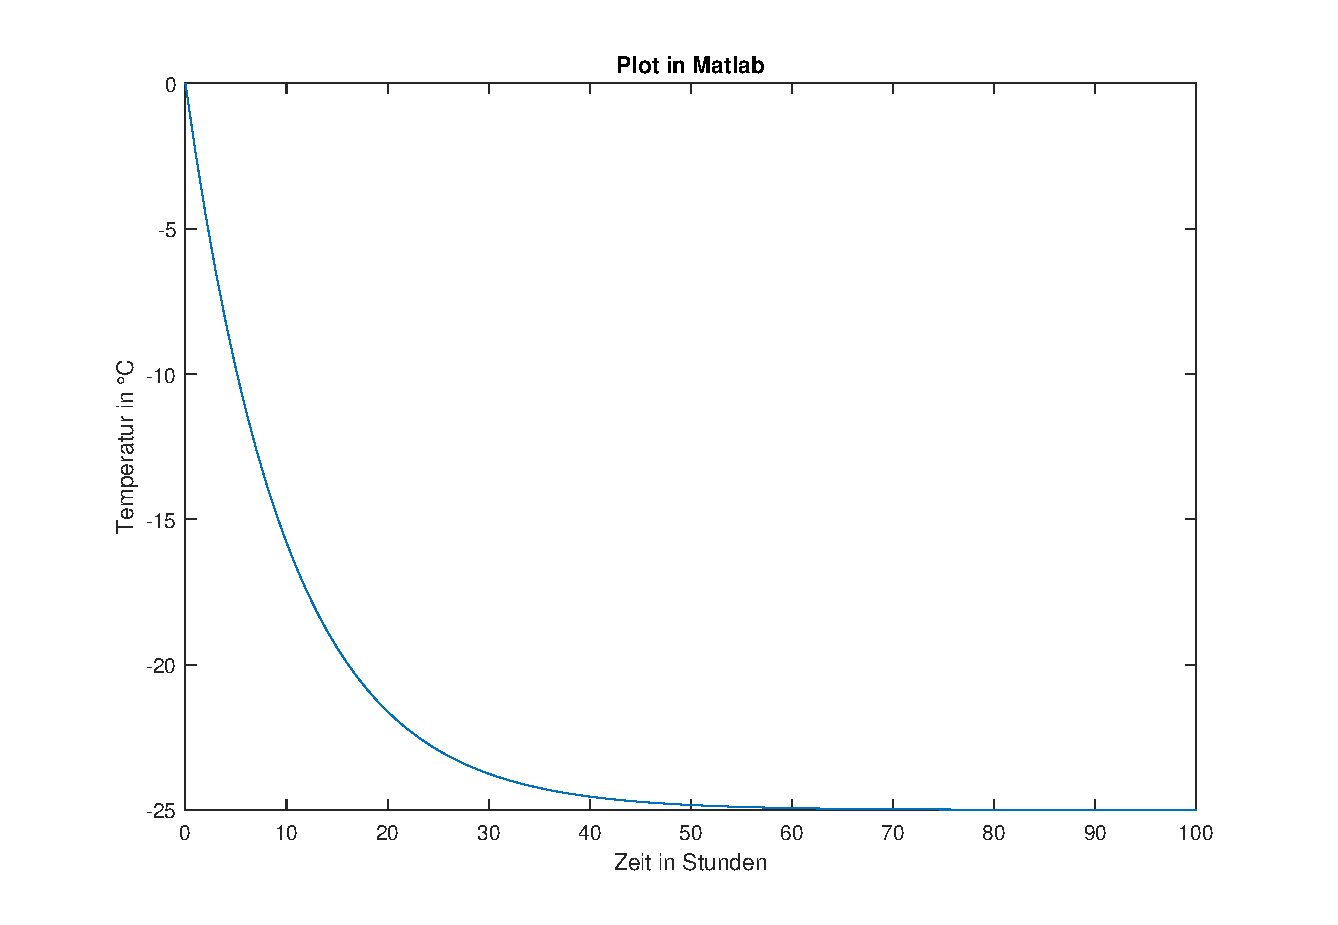
\includegraphics[width=12cm]{images_2/Übergangsfunktion/Übergangsfkt_plot_matlab.eps}
    \caption{Sprungantwort: Plot mit Matlab}
\end{figure}

\subsubsection{Plot mit Step-Funktion}
Den selben Plot erhält man in Matlab auch über die \texttt{step}-Funktion. Diese lässt sich durch folgende Befehle anzeigen:\\
\hspace*{0.5cm}\texttt{sys = tf([-25],[10 1])}\\
\hspace*{0.5cm}\texttt{step(sys)}\\
Das von Matlab gelieferte Ergebnis ist in Abbildung 2 dargestellt.
\begin{figure}[H]
    \centering
    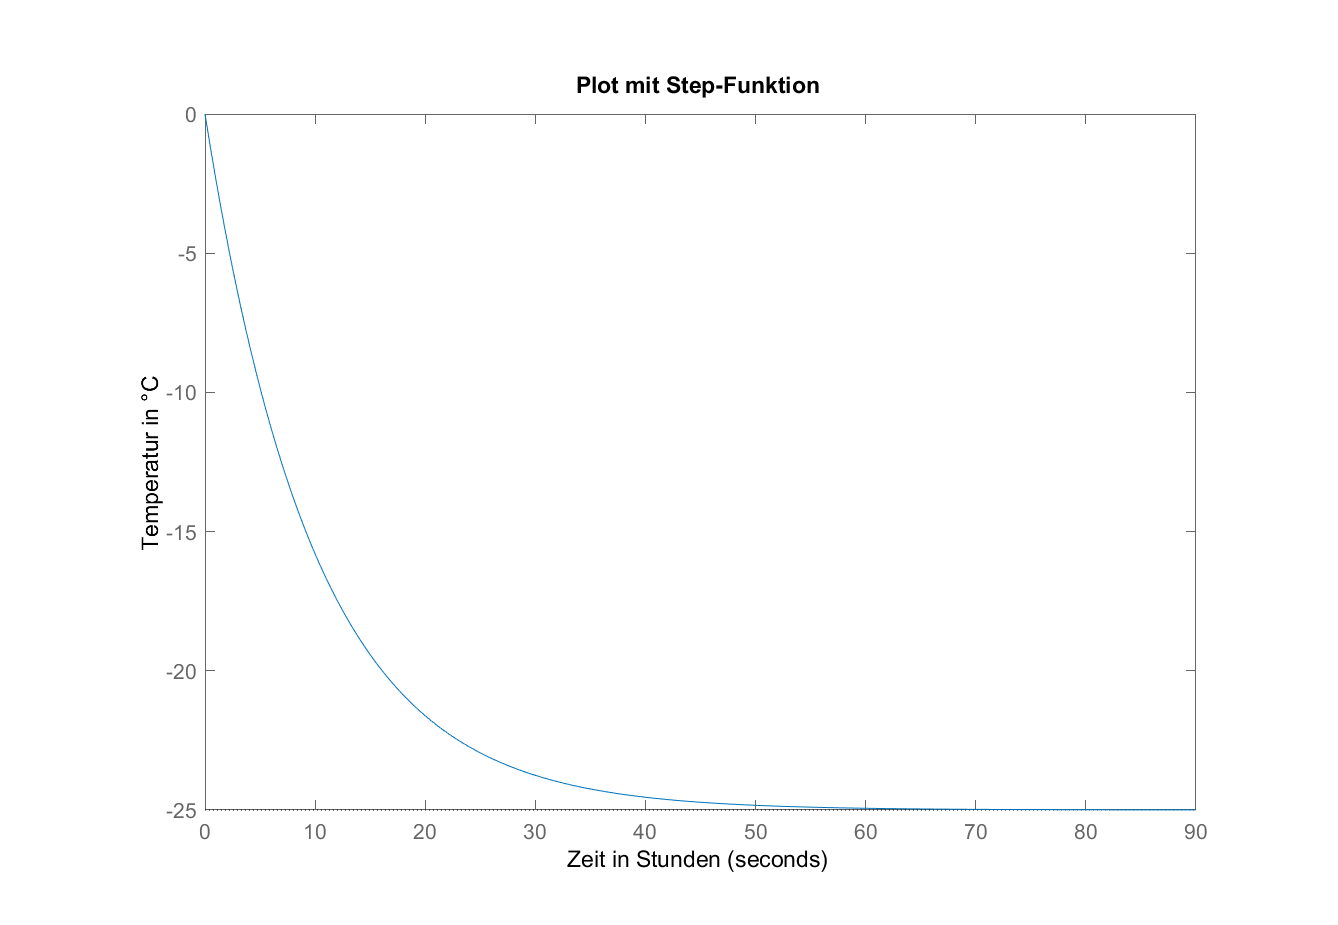
\includegraphics[width=12cm]{images_2/Übergangsfunktion/Übergangsfkt_plot_stepfunktion.eps}
    \caption{Sprungantwort: Plot mit Step-Funktion}
\end{figure}

\subsubsection{Plot mit Simulink}
Das selbe Ergebnis lässt sich ebenfalls in Simulink durch folgende Schaltung erzielen:
\begin{figure}[H]
    \centering
    \includegraphics[width=13cm]{images_2/Übergangsfunktion/simulink-schaltung.png}
    \caption{Sprungantwort: Simulink Schaltung}
\end{figure}
\begin{figure}[H]
    \centering
    \includegraphics[width=10cm]{images_2/Übergangsfunktion/übergangsfkt_simulink-plot.png}
    \caption{Sprungantwort: Plot mit Simulink}
\end{figure}












% Da t ein Vektor ist, muss man beim Multiplizieren das Punktprodukt (Hadammad-Produkt) verwenden.

        
%Die Control System Toolbox dient der systematischen Analyse, dem Entwurf und der Optimierung linearer Systeme.\\
%Mit dem folgenden Matlab-Skript kann ich die Übertragungsfunktion G(s) in MATLAB eingeben.
%\lstinputlisting[style=Matlab-editor, caption={pretty}]{../MATLAB/ControlSystemToolbox/cst_DTs.m}
%Lässt man sich G(s) in der Konsole anzeigen, wird diese folgendermaßen dargestellt.
                    
%Durch den Befehl \texttt{step(sys)} öffnet MATLAB ein neues Fenster mit der passenden Sprungantwort h(s) zu G(s) und stellt diese folgendermaßen dar.




\vspace*{1cm}


\section{Gewichtsfunktion/Impulsantwort}
%Antwort auf einen Delta-Impuls.
%Die Lösung von Matlab ist zwar die gleiche, aber in einer anderen Darstellung. Sollte Matlab einen zu langen Ausdruck ausgeben, kann der Befehl simplify(ans) verwendet werden, um den Ausdruck zu vereinfachen.

\subsection{Parametrische Darstellung} %NICHT SICHER
Die parametrische Darstellung der Gewichtsfunktion $g(t)$ erhält man, indem man die Laplace-Rücktransformierte der Übertragungsfunktion bildet. Das macht man in Matlab durch folgende Befehle:\\
%syms s -> G(s)=bspw. 3*s/(1+9*s + 20*s^2) -> ilaplace(G(s)) -> t=[0;0.1;10] -> plot(t, Antwort der parametrischen Darstellung) (Da t ein Vektor ist, muss man beim Multiplizieren das Punktprodukt (Hadamad-Produkt) .* verwenden) (Alternativ kann man das mit dem fplot befehl machen, da spart man sich das Hadamad-Produkt) -> xlabel (Mit den Befehlen xlabel und ylabel kann man die Achsen beschriften) -> ylabel Gewichtsfunktion
\hspace*{0.5cm}\texttt{syms s t}\\
\hspace*{0.5cm}\texttt{G(s)=-25/(10*s+1)}\\
\hspace*{0.5cm}\texttt{g(t)=ilaplace(G(s))}\\
Alternativ lässt sich die Gewichtsfunktion auch durch Ableiten der Übertragungsfunktion $h(t)$ berechnen. In Matlab lässt sich das durch den Befehl \texttt{g(t) = diff(h(t))} bewerkstelligen.\\\\
In beiden Fällen liefert Matlab das Ergebnis:
\begin{equation*}
    g(t)=-\frac{5*e^{\frac{-t}{10}}}{2}
\end{equation*}

\subsection{Nichtparametrische Darstellung}
\subsubsection{Plot mit Matlab}
Nach der Berechnung der Gewichtsfunktion $g(t)$ lässt sich diese durch folgende Befehle in Matlab plotten:
\texttt{t=[0:1:100]}\\
\texttt{t, g(t)}\\
Das von Matlab gelieferte Ergebnis ist in der folgenden Abbildung dargestellt:
\begin{figure}[H]
    \centering
    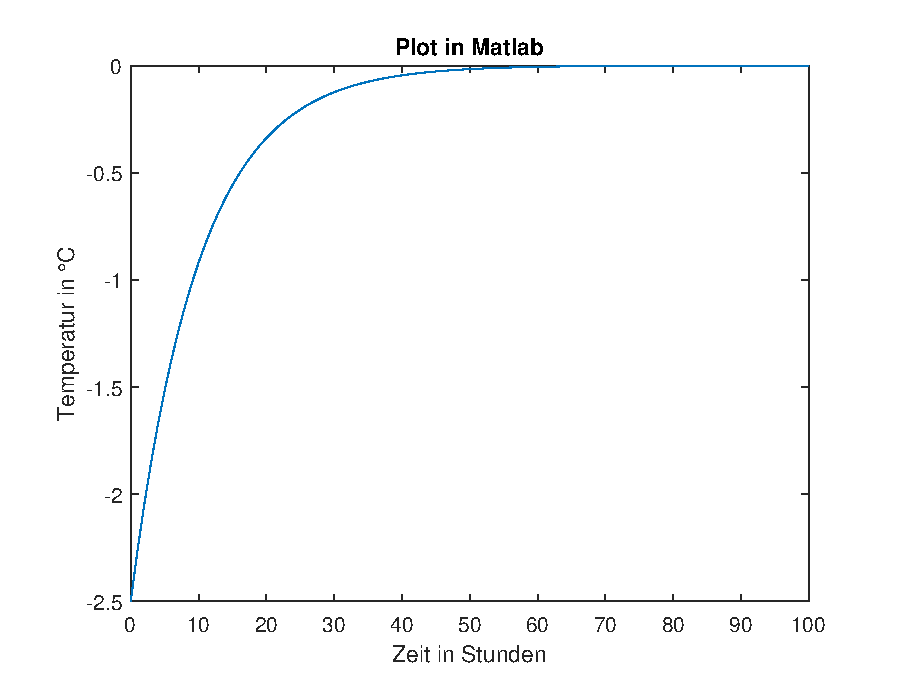
\includegraphics[width=10cm]{images_2/Gewichtsfunktion/gewichtsfkt_plot_mit_matlab.eps}
    \caption{Impulsantwort: Plot in Matlab}
\end{figure}

\subsubsection{Plot mit Step-Funktion}
Den selben Plot erhält man in Matlab auch über die \texttt{impulse}-Funktion. Diese lässt sich durch folgende Befehle anzeigen:\\
\hspace*{0.5cm}\texttt{sys = tf([-25],[10 1])}\\
\hspace*{0.5cm}\texttt{impulse(sys)}\\
Das von Matlab gelieferte Ergebnis ist in der folgenden Abbildung dargestellt.
\begin{figure}[H]
    \centering
    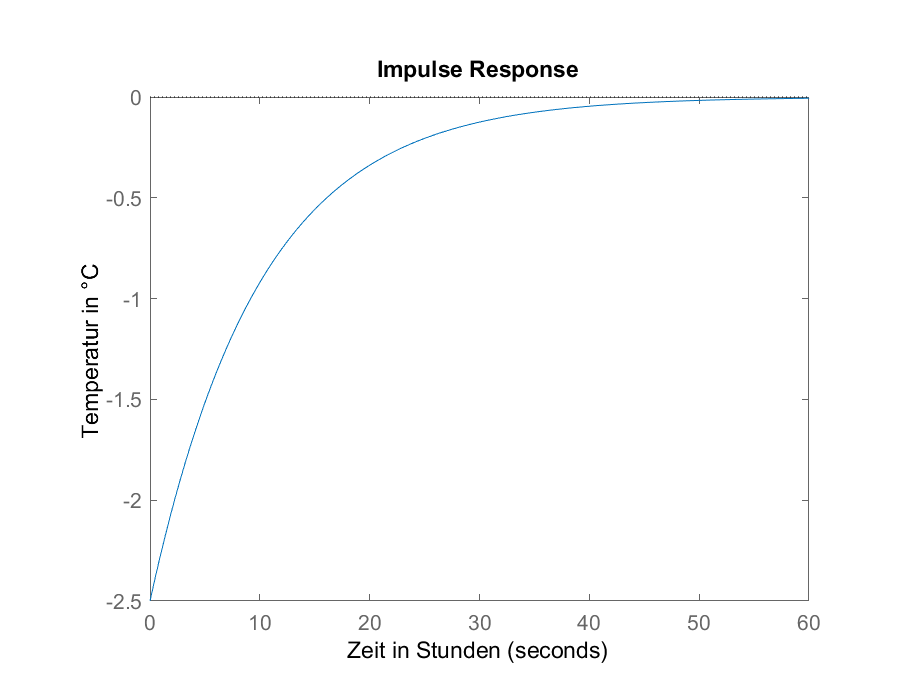
\includegraphics[width=10cm]{images_2/Gewichtsfunktion/gewichtsfkt_impulse.eps}
    \caption{Impulsantwort: Plot mit \texttt{impulse}-Funktion}
\end{figure}

\subsubsection{Plot mit Simulink}
Das Ergebnis eines Deltaimpulses kann in Simulink simuliert werden, indem die Übertragungsfunktion mit $s$ multipliziert wird. Die Simulink-Schaltung und der dazu gehörige Plot sehen wie folgt aus:
\begin{figure}[H]
    \centering
    \includegraphics[width=12cm]{images_2/Gewichtsfunktion/impuls_simulink_schaltung.png}
    \caption{Impulsantwort: Simulink-Schaltung}
\end{figure}
\begin{figure}[H]
    \centering
    \includegraphics[width=10cm]{images_2/Gewichtsfunktion/impulsantwort_simulink.png}
    \caption{Impulsantwort: Plot mit Simulink}
\end{figure}

\vspace*{1cm}


\section{Frequenzgang}
Den Frequenzgang erhält man indem man die komplexe Variable $s$ durch iOmega ($i\omega$) ersetzt. \\
Das ist gleichbedeutend mit einem Schnitt der komplexen Funktion $G(s)$ entlang der imaginären Achse.
Damit wird jeder Kreisfrequenz $\omega$ eine komplexe Zahl $G(i\omega)$ zugeordnet. 
\\
\\
Bedingt durch den Schnitt hat der Frequenzgang eine geringere Aussagekraft als die Übertragungsfunktion. 
Die Bedeutung des Frequenzgangs ergibt sich aus der Tatsache, dass das stationäre Verhalten des Systems auf eine sinuidale Anregung beschrieben wird.\\
\\

Sei $u(t) = sin(\omega t)$, so ist $y_{stat}(\dot{t})$ %TODO: KONTROLLE
, dh. das Ausgangssignal nach Abklingen der Anfangswerte durch:
\begin{equation*}
    y_{stat}(t)=A*|G(i\omega )|sin(\omega t + \phi (G(i\omega )))
\end{equation*}

gegeben. %TODO: KONTROLLE und Block
%Der Frequenzgang liefert formal weniger Aussagen als die Übertragungsfunktion, da er nicht alle $s$ betrachtet, sondern nur die $s$, die auf der imaginären Achse liegen.\\
%Experimentell könnte der Frequenzgang durch die folgende Simulink-Schaltung aufgenommen werden. 
%TODO: Schaltung einfügen
%Man stellt eine Frequenz ein und schaut am Ausgang die Amplitudenverstärkung und die Phasenverschiebung an. Hat der Eingangssinus die Amplitude 1, kann ich die Verstärkung am Ausgang direkt ablesen. Den erhaltenen Punkt trägt man in das Bode-Diagramm ein. Danach wiederholt man das Experiment mit einer anderen Frequenz. Hat man genügend Punkte, so verbindet man diese und erhält das Bode-Diagramm. Ebenso wie wir an den Verläufen der Sprungantwort auf die Differentialgleichung schließen konnten, können Experten aus den Verläufen des Bode-Diagramms auf den Frequenzgang (und damit auf die Übertragungsfunktion und damit auf die Differentialgleichung) schließen.\\
%Die Phasenverschiebung kann selbstverständlich auch mit Computeralgebra ausgerechnet werden.
\subsection{Parametrische Darstellung}
Experimentell kann der Frequenzgang durch folgende Simulink Schaltung aufgenommen werden:
 
\subsection{Nichtparametrische Darstellung}
\subsubsection{Nyquist-Plot (Ortskurve)}
%Realteil von G(iw)
...
\subsubsection{Bode-Plot}
...

\vspace*{1cm}


\section{Pol-Nullstellen-Plot}
Der Pole-Zero-Plot stellt die Pole und Nullstellen der Übertragungsfunktion in der komplexen Ebene dar. Pole werden durch ein Kreuz dargestellt, Nullstellen durch einen Kreis. Ein Doppelpol wird durch ein Doppelkreuz und eine Nullstelle durch einen Doppelkreis dargestellt. Der PZP enthält keine Informationen mehr über die statische Verstärkung. Aus dem PZP lassen sich Eigenschaften wie Stabilität und Minimalphasigkeit ablesen. So ist ein System stabil, wenn alle Pole in der linken offenen Halbebene liegen. Es ist instabil, sobald ein Pol auf der rechten Halbebene liegt. Es ist grenzstabil, wenn keine Pole in der rechten Halbebene liegen aber einige auf der imaginären Achse liegen. Ein System ist minimalphasig, wenn alle Nullstellen in der offenen linken Halbebene liegen. Es ist nicht minimalphasig, sobald eine Nullstelle auf der rechten Halbebene liegt. Und letztlich ist es schwachminimalphasig, wenn keine Nullstelle auf der rechten Halbebene liegt, aber Nullstellen auf der imaginären Achse auftauchen.


\section{Statische Kennlinie}
In der statischen Kennlinie wird der Ausgang über dem Eingang dargestellt. 
Bei einem linearen System (unten $u$ oben $y$) ist die statische Kennlinie eine Ursprungsgerade, deren Anstieg der statischen Verstärkung entspricht. 
Die statische Verstärkung $K$ kann aus $G(0)=K$ berechnet werden. Sie ist bei Systemen mit D-Verhalten 0 und bei Systemen mit I-Verhalten unendlich. 
Mit anderen Worten, Systeme mit I-Verhalten haben keine Kennlinie. In der statischen Kennlinie ist keinerlei Dynamik zu erkennen. 
Die Information über Pole, Nullstellen, etc. fehlt. Sie ist somit die schwächste der Modellbeschreibungen. 
Gleichwohl ist sie einfach zu bestimmen. Man stellt einen konstanten Wert $u$ ein, wartet bis die Eigenvorgänge abgeklungen 
%(bis es eingeschwungen ist) 
sind und liest den $y$-Wert ab. Diesen Punkt trägt man in das Diagramm ein und wiederholt das ganze für mehrere Punkte. In der Praxis werden sich häufig nicht ideale Geraden ergeben. Bei Öfen verringert sich der Anstieg beispielsweise bei hohem $u$. Der Praktiker ließt aus der statischen Kennlinie ab, wie gut seine Annahme eines linearen Modells ist. Sie ist gut in einem Bereich, in dem eine Geradenapproximation akzektabel ist (wenn sie einer Gerade ähnelt). Bei einem Mehrgrößensystem mit zwei Eingängen und zwei Ausgängen wählt man häufig die folgende Darstellung: Entweder zwei Einzeldiagramme, oder ein Verbunddiagramm (zwei Eingänge ein Ausgang: Üblicherweise keine 3D-Darstellung, sondern Transistorkennlinien). Bei Systemen mit zwei Eingängen 
%wird häufig eine Eingangsvariable durch Kennlinienscharen diskretisiert/
wählt man häufig die Darstellung mit Kennlinienscharen, wobei beispielsweise $u_{1}$ die reellen Zahlen darstellt und $u_{2}$ den Scharparameter darstellt.
%Indem man alle Ableitungen gleich Null setzt und eine Beziehung zwischen den y und u herstellt. Gegebenenfalls muss x eliminiert werden (lineares Gleichungssystem).
\end{document}





%TODO: Linearisierung:
%Nachdem man die Ruhelagen berechnet hat kann man um jede einzelne Ruhelage das System linearisieren. In der Folge entsteht ein lineares System, welches für kleine Abweichungen um die Ruhelage Gültigkeit hat. Man nennt dieses auch die Variationsgleichung oder einfach auch linearisiertes System. Das linearisierte System ist deutlich einfacher zu behandeln, da sich z.B. über Eigenwerte Aussagen zur Stabilität der Ruhelage treffen lassen. Vorgehen:
%Im Falle eines SiSo-Systems ist f(x) die Jacobi-Matrix an der Ruhelage und f_u der Eingangsvektor.